\documentclass[12pt, letterpaper] {article}

\parindent=5mm
\usepackage[spanish]{babel}

\usepackage{amssymb}
\usepackage{amsmath} 
\usepackage{amsfonts}

\usepackage[numbers,sort&compress]{natbib}
\usepackage{graphicx}

\usepackage{url}
\usepackage{hyperref}

\usepackage[top=25mm, bottom=20mm, left=1.5cm, right=1.5cm]{geometry}
\setlength{\parskip}{2mm}
\setlength{\parindent}{1pt}

\usepackage{listings}

\usepackage{float}

\usepackage[utf8]{inputenc}
\usepackage{graphicx} 
\usepackage{subfigure} 

\usepackage{color}
\usepackage{multirow}

\definecolor{dkgreen}{rgb}{0,0.6,0}
\definecolor{gray}{rgb}{0.5,0.5,0.5}
\definecolor{mauve}{rgb}{0.58,0,0.82}

\usepackage{color}
\usepackage{listings}
\lstset{ %
  language=R,                     % the language of the code
  basicstyle=\footnotesize,       % the size of the fonts that are used for the code
  numbers=left,                   % where to put the line-numbers
  numberstyle=\tiny\color{gray},  % the style that is used for the line-numbers
  stepnumber=1,                   % the step between two line-numbers. If it's 1, each line
                                  % will be numbered
  numbersep=5pt,                  % how far the line-numbers are from the code
  backgroundcolor=\color{white},  % choose the background color. You must add \usepackage{color}
  showspaces=false,               % show spaces adding particular underscores
  showstringspaces=false,         % underline spaces within strings
  showtabs=false,                 % show tabs within strings adding particular underscores
  frame=single,                   % adds a frame around the code
  rulecolor=\color{black},        % if not set, the frame-color may be changed on line-breaks within not-black text (e.g. commens (green here))
  tabsize=2,                      % sets default tabsize to 2 spaces
  captionpos=b,                   % sets the caption-position to bottom
  breaklines=true,                % sets automatic line breaking
  breakatwhitespace=false,        % sets if automatic breaks should only happen at whitespace
  title=\lstname,                 % show the filename of files included with \lstinputlisting;
                                  % also try caption instead of title
  keywordstyle=\color{blue},      % keyword style
  commentstyle=\color{dkgreen},   % comment style
  stringstyle=\color{mauve},      % string literal style
  escapeinside={\%*}{*)},         % if you want to add a comment within your code
  morekeywords={*,...}            % if you want to add more keywords to the set
} 

\author{Ricardo Rosas Macías}

\title{Práctica 9: interacciones entre partículas}

\date{\today}

\begin{document}

\maketitle


\section{Introducción}
En la práctica se muestra la interacción de partículas que tienen un movimiento en función a las cargas, de manera que las partículas crean fuerzas de atracción y repulsión entre ellas al estar cerca de su campo. 

 \section{Objetivo}
Se realizó cambios en el c\'odigo proporcionado en la p\'agina web \cite{elisawebIEP}, de tal forma que el movimiento de las partículas esta ligado a la masa que esta posee, de modo que emule a una fuerza de tipo gravitacional; resultando una manifestación de atracción entre ellas. 
 
 \subsection{Descripción}
 
La finalidad del experimento es \cite{elisawebIEP}:
\begin{quotation}
 ``Agregar a cada partícula una masa y hacer que la masa cause fuerzas gravitacionales (atracciones) además de las fuerzas causadas por las cargas. Asimismo, estudiar la distribución de velocidades de las partículas y verifica gráficamente que esté presente una relación entre los tres factores: la velocidad, la magnitud de la carga, y la masa de las partículas.''
\end{quotation}

\section{Resultados y conclusiones}

En base al trabajo anteriormente reportado \cite{PG9}\cite{MP9}, se realizó el código que se muestra en la parte inferior. En las primeras líneas del c\'odigo se defini\'o los par\'ametros de experimentaci\'on con las cuales se trabajó, además se creó una masa para todas partículas que posteriormente tendrá un efecto en la interacción con todas las que se encuentren en su alrededor, igualmente se estableció parámetros para que dicha masa sea una fuerza más en el experimento. 

\begin{lstlisting}[language=R]
n <- 50
p <- data.frame(x = rnorm(n), y=rnorm(n), c=rnorm(n),m=rnorm(n))
p$m <- abs(p$m)
\end{lstlisting}


De acuerdo a lo anteriormente mencionado, esta masa efectuará cambios positivos en la carga de la partícula. Por lo tanto en las siguientes líneas de código se muestra el efecto que tendrá la masa de la partícula tanto a la fuerza gravitacional entre todas las partículas así como el cambio en la velocidad por dicho fenómeno durante los 100 pasos posteriormente declarados.

\begin{lstlisting}[language=R]
  mi <- p[i,]$m 
  
  pi<-cbind(p$x,p$y)
  pi<-data.frame(pi)
  colnames(pi)<-c(``x'',``y'')

disx<- pi$x - p$x
  disy<- pi$y - p$y
  v<-sqrt(disx^2 + disy^2)
  res<-cbind(p$m,v)
  datos<-rbind(datos,res)

 ggplot() +
    geom_point(data=p, aes(x = p$x, y= p$y,size=p$m,color=p$g))+
    scale_x_continuous(name="x",limits = c(0, 1))+
    scale_y_continuous(name="y", limits = c(0, 1))+
    scale_colour_manual(values=colores)+  
    ggtitle(paste("Paso",iter))+
    theme(plot.title = element_text(hjust = 0.5))+
    guides(size=FALSE,color=guide_legend(title="Carga"))+
    theme(axis.text.x=element_text(size=12),
          axis.text.y=element_text(size=12),
          plot.title=element_text(size=14),
          axis.title.x = element_text(size=12),
          axis.title.y = element_text(size=12))
  ggsave(paste("P9_t",iter,".png", sep=""))
  
}
stopImplicitCluster()

datos$n<-seq(1,n,1)
colnames(datos)<-c("Masa","Velocidad","n")
tabla<-data.frame()

for (i in 1:n){
  res<-datos[datos$n==i,]
  resultados<-cbind(res[i,]$Masa,mean(res$Velocidad))
  tabla<-rbind(tabla,resultados)
}
colnames(tabla)<-c("Masa","Velocidad")

ggplot(tabla, aes(x=Masa, y=Velocidad))+
  geom_point(shape = 17, color = "#FC4E07", size = 1.7)+
  geom_smooth(method = "lm", formula =y ~log(x))+
  scale_x_continuous(name="Masa")+
  scale_y_continuous(name="Velocidad")
ggsave("Veldep.png")\end{lstlisting}


Con ayuda de la paquetería \textit{Lattice} se obtuvo la visualización de la ejecución del código, como se muestra en la figura \ref{SimF}, con la cual se determina que el código creado realmente si cumple con el objetivo planteado. Se observa que al generar las partículas muchas empiezan a interactuar con sus vecinas de manera que ocasionan una convergencia para todas las partículas.

\begin{figure}[H]
\centering
\subfigure[Generadas]{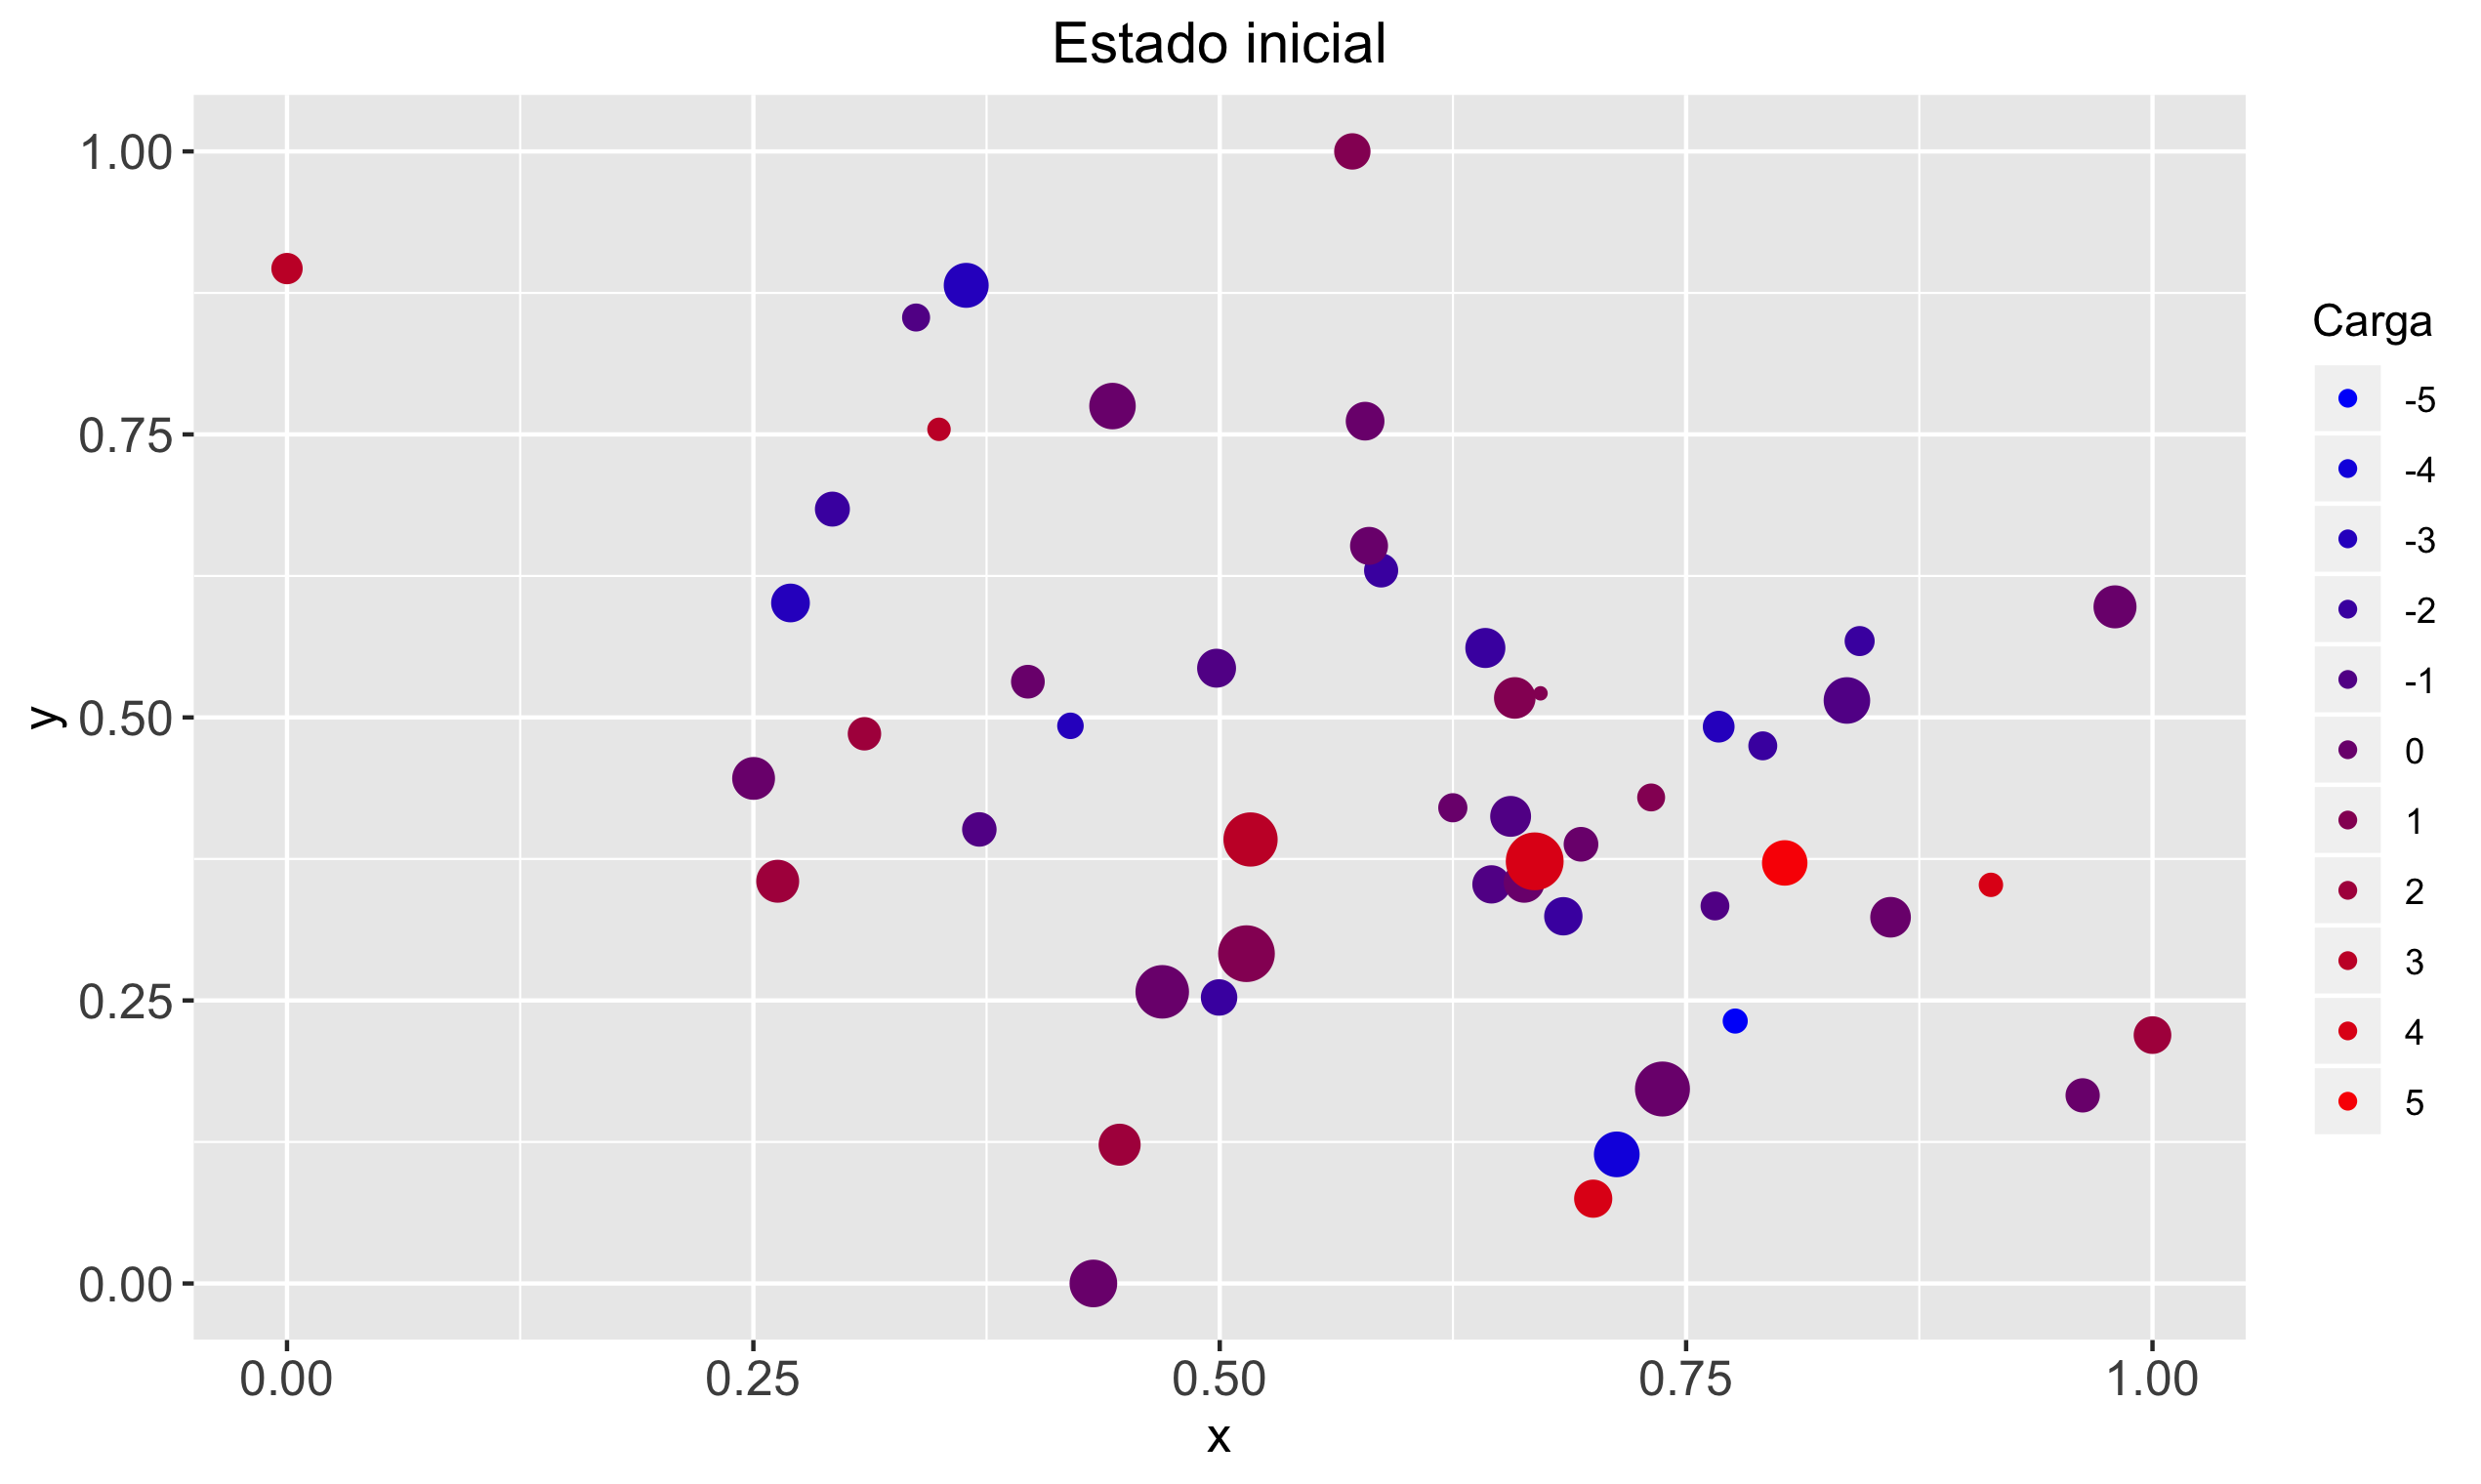
\includegraphics[width=75mm]{./p9_t0}}\vspace{1mm}
\subfigure[Primer paso]{\includegraphics[width=75mm]{./p9_t1}}
\subfigure[Paso 25]{\includegraphics[width=75mm]{./p9_t25}}
\subfigure[Paso 50]{\includegraphics[width=75mm]{./p9_t50}}
\subfigure[Paso 75]{\includegraphics[width=75mm]{./p9_t75}}
\subfigure[Paso 100 ]{\includegraphics[width=75mm]{./p9_t100}}
\caption{Atracción de partículas en la simulación}\label{SimF}
\end{figure}

Para estudiar la distribución de velocidades las partículas se obtuvieron histogramas como se puede observar en la figura \ref{Hist}, que permiten ver una normalización de la velocidad respecto a la distancia recorrida por la interacción de las cargas de las partículas.

\begin{figure}[H]
\centering
\subfigure[Paso 1]{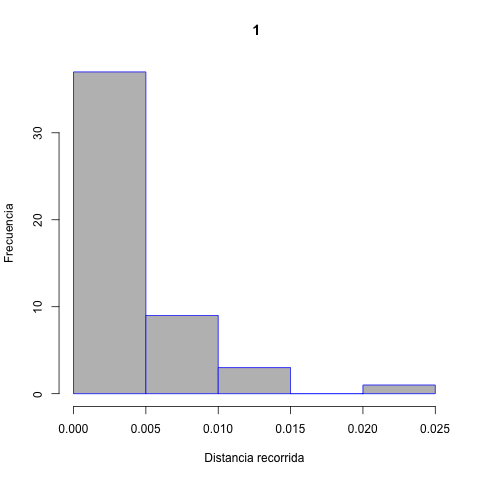
\includegraphics[width=56mm]{./histo1}}\vspace{0mm}
\subfigure[Paso 25]{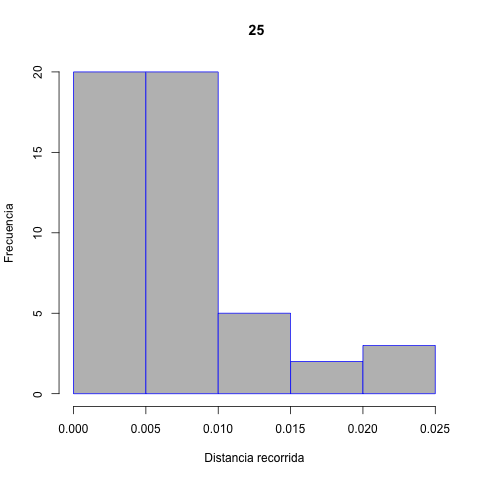
\includegraphics[width=56mm]{./histo25}}
\subfigure[Paso 50]{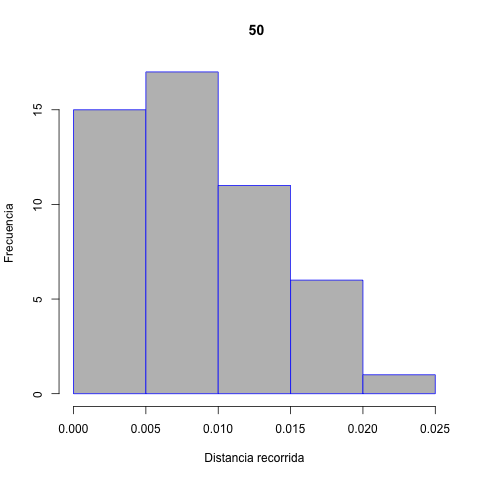
\includegraphics[width=56mm]{./histo50}}
\subfigure[Paso 50]{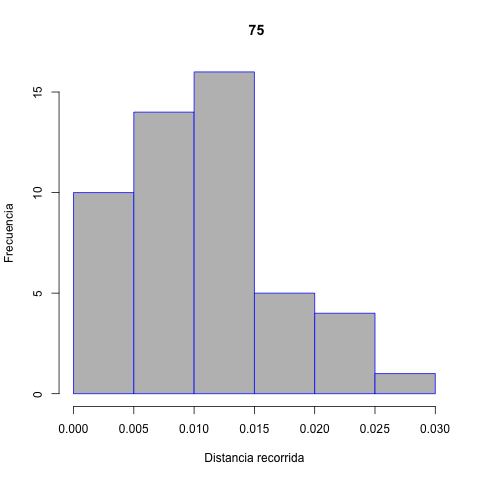
\includegraphics[width=56mm]{./histo75}}
\subfigure[Paso 100]{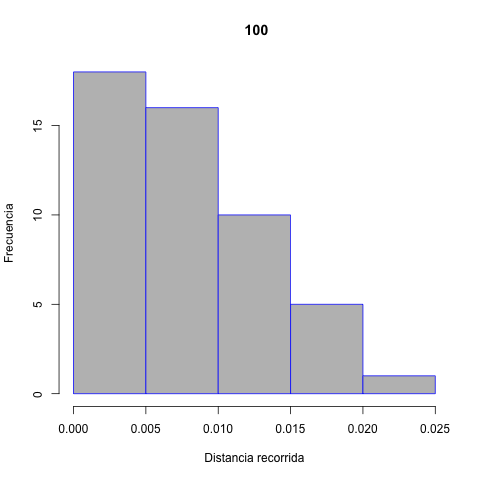
\includegraphics[width=56mm]{./histo100}}
\caption{Distancia de partículas}\label{Hist}
\end{figure}

Por último se obtuvo la figura \ref{VelMasa}  para ver de manera más puntual la distribución mencionada en la sección anteriormente, en donde se evidencía que conforme avanza el número movimientos respecto a la velocidad de los pasos establecidos; estos van disminuyendo, de forma que indica que el experimento se mantiene estable, sin afectar drásticamente con un rechazo por las cargas iguales. 

\begin{figure}[H]
\centering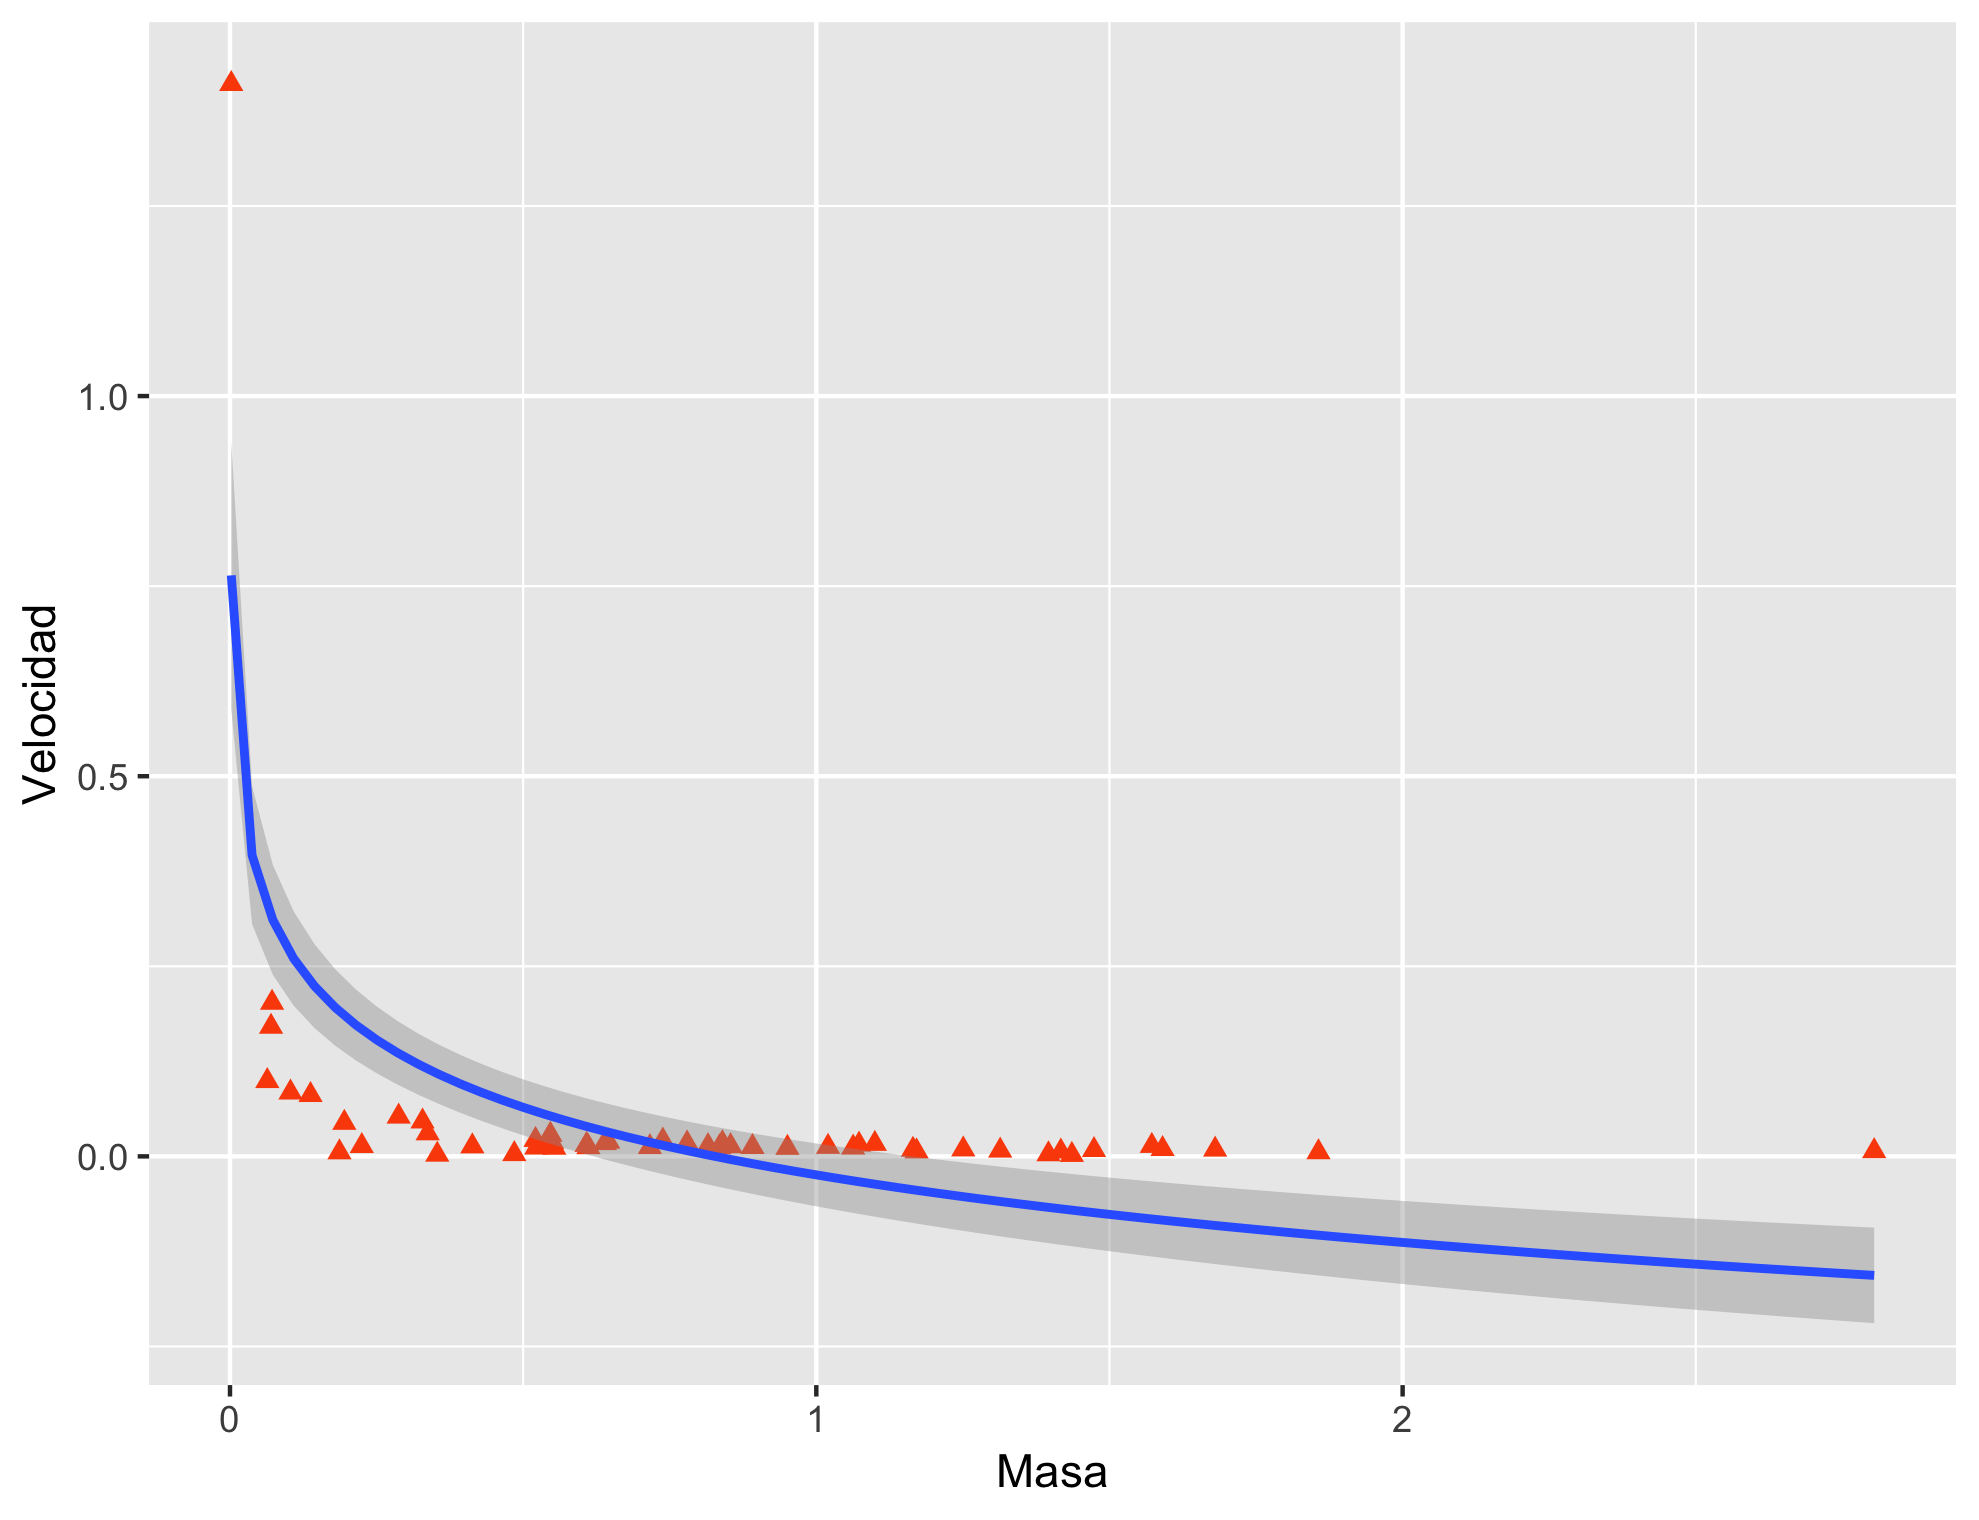
\includegraphics[width=108mm]{Veldep.png}
\caption{Vel respecto a la masa de las partículas}
\label{VelMasa}
\end{figure}



\bibliographystyle{plainnat}

\bibliography{BiblioHWP9}

\end{document}